\section{Numerical Experiments}
\label{sec:experiments}

We evaluate our (Nested) WAIT algorithm through numerical experiments. Our analysis focuses on two distinct scenarios: (i) simulated prompts designed to test the algorithm under controlled conditions, and (ii) a real-world dataset sourced from \cite{zheng2023lmsys} to assess its performance in practical settings.

We conduct all experiments using Microsoft Vidur to simulate an NVIDIA A100 GPU, mirroring the hardware configuration that prior studies used \citep{agrawal2024vidur}. We benchmark our WAIT algorithm against vLLM \citep{kwon2023efficient} and Sarathi \citep{agrawal2023sarathi}, widely recognized inference engines that employ First-Come-First-Serve (FCFS) scheduling. Specifically, vLLM prioritizes new arrivals, while Sarathi prioritizes ongoing prompts, with both enforcing fixed limits on the total number of tokens and prompts per iteration.

\subsection{Experiment on WAIT Algorithm}
We first evaluate the WAIT algorithm when prompt output lengths are known upon arrival. We generate simulated prompts with varying input lengths \( l_j \) and output lengths \( l_j' \), drawn from distributions that emulate real-world variability. We adjust arrival rates \( \lambda_j \) to simulate both low-traffic and high-traffic scenarios, testing the algorithm's resilience under stress. Specifically, we generate type \( j \) prompts via a Poisson process with rate \( \lambda_j \) and test two scenarios:

(i) \textbf{Low demand}: \( m=2 \), \( (l_1, l_2) = (10, 10) \), \( (l_1', l_2') = (10, 20) \), \( (\lambda_1, \lambda_2) = (1000, 1000) \);  

(ii) \textbf{High demand}: \( m=3 \), \( (l_1, l_2, l_3) = (20, 20, 20) \), \( (l_1', l_2', l_3') = (100, 200, 300) \), \( (\lambda_1, \lambda_2, \lambda_3) = (6000, 4000, 2000) \).

For practical implementation, we simplify threshold computation in WAIT. Given a batch size limit \( B \), we set the threshold for type \( j \) prompts as \( n_j = B \cdot \rho_j / (l_j' + 1) \), where \( \rho_j = \lambda_j / \sum_{j'=1}^m \lambda_{j'} \), aligning with Algorithm \ref{alg:wait}. To ensure a fair comparison, we enforce the same batch size limit across WAIT, Sarathi, and vLLM.

The throughput of WAIT surpasses that of the benchmark algorithms across all tested arrival rates, as illustrated in the left panels of Figure~\ref{fig:comparison WAIT short decode} and Figure~\ref{fig:comparison WAIT long decode}. This improvement is due to WAIT's ability to optimize batch formation, minimizing GPU idle time. Latency, shown in the right panels, remains within acceptable limits, indicating a good balance between efficiency and responsiveness.

\begin{figure}[htbp]
    \centering
    \begin{minipage}{0.4\textwidth}
        \centering
        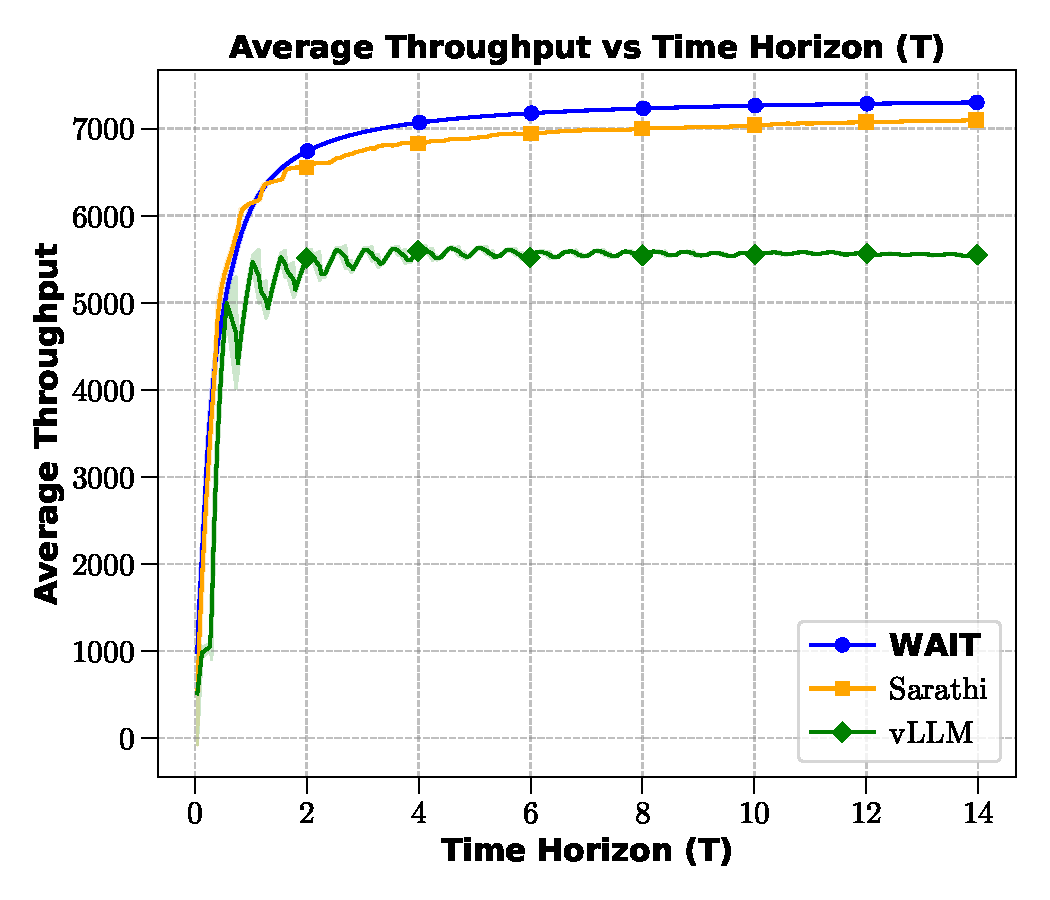
\includegraphics[width=\textwidth]{Experiments_pdf/test9_simulated_short_decode_throughput.pdf}
    \end{minipage}
    \hfill
    \begin{minipage}{0.4\textwidth}
        \centering
        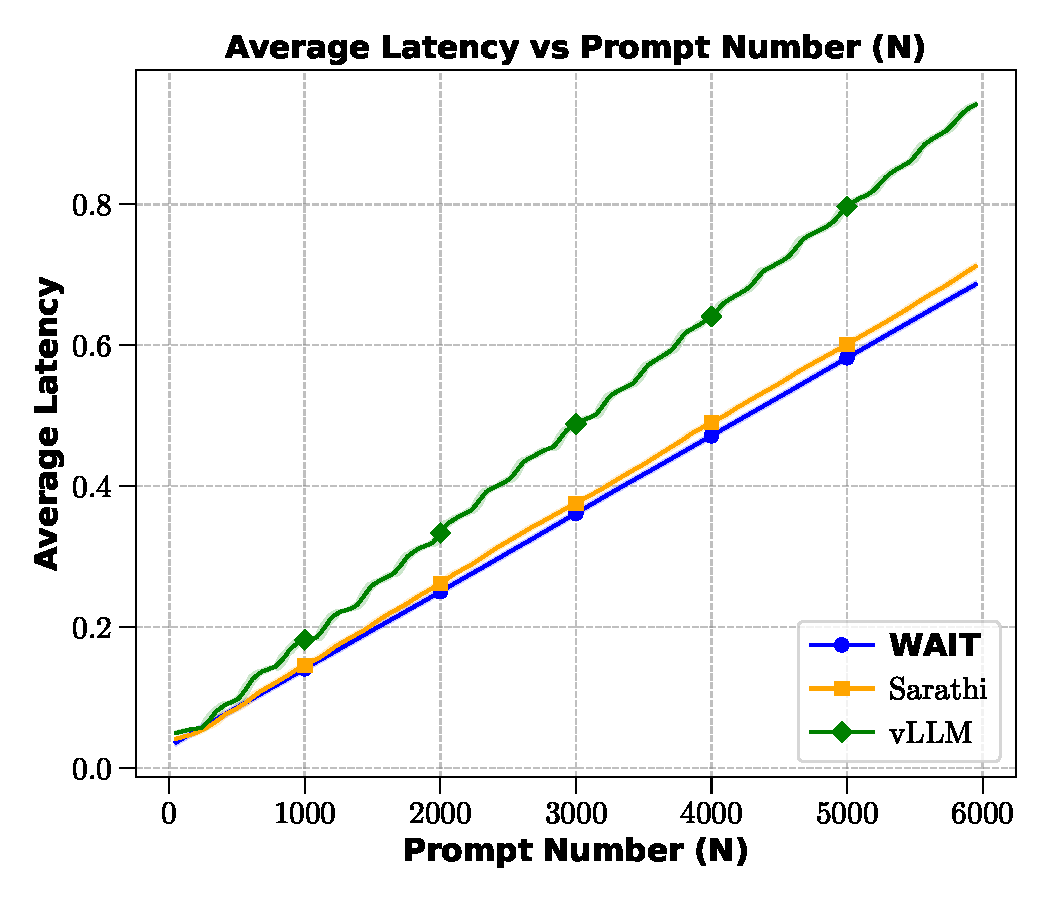
\includegraphics[width=\textwidth]{Experiments_pdf/test9_simulated_short_decode_latency.pdf}
    \end{minipage}
    \caption{Average throughput and latency across algorithms on the synthetic dataset with low demand.}
    \label{fig:comparison WAIT short decode}
\end{figure}

\begin{figure}[htbp]
    \centering
    \begin{minipage}{0.4\textwidth}
        \centering
        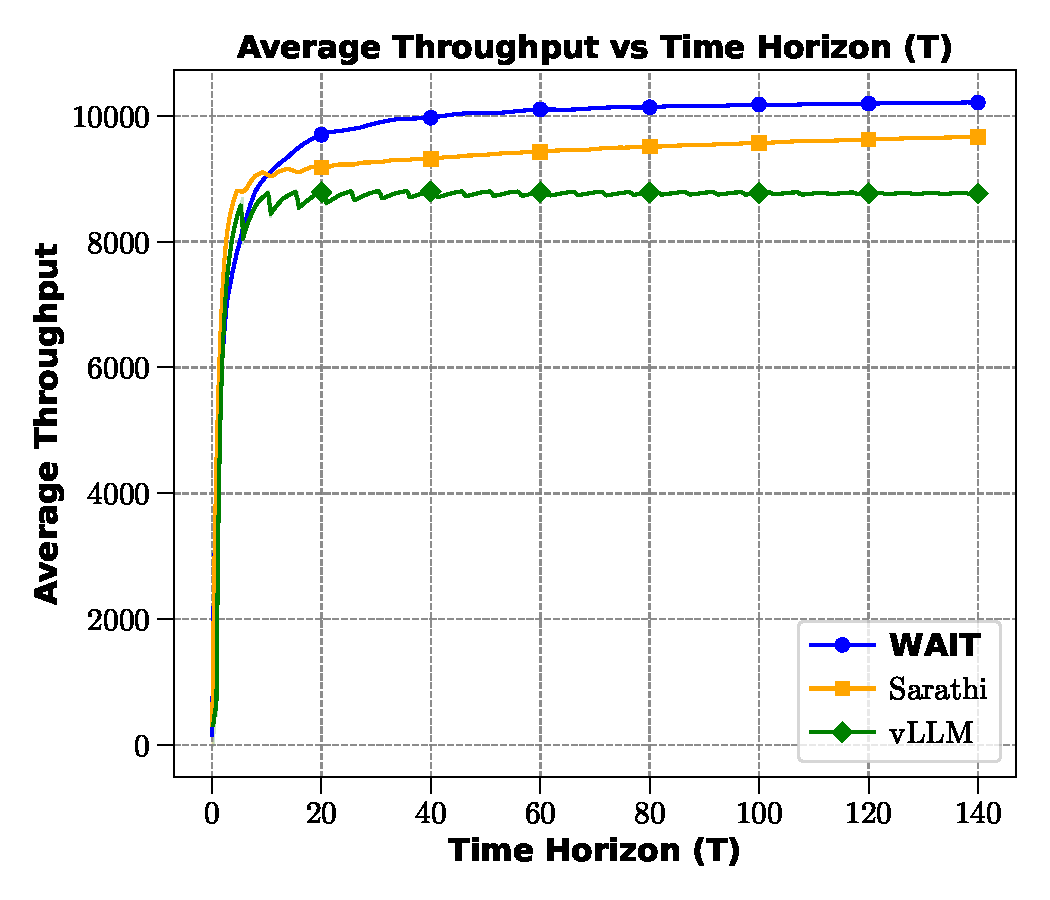
\includegraphics[width=\textwidth]{Experiments_pdf/test13_simulated_short_decode_bs=448_throughput.pdf}
    \end{minipage}
    \hfill
    \begin{minipage}{0.4\textwidth}
        \centering
        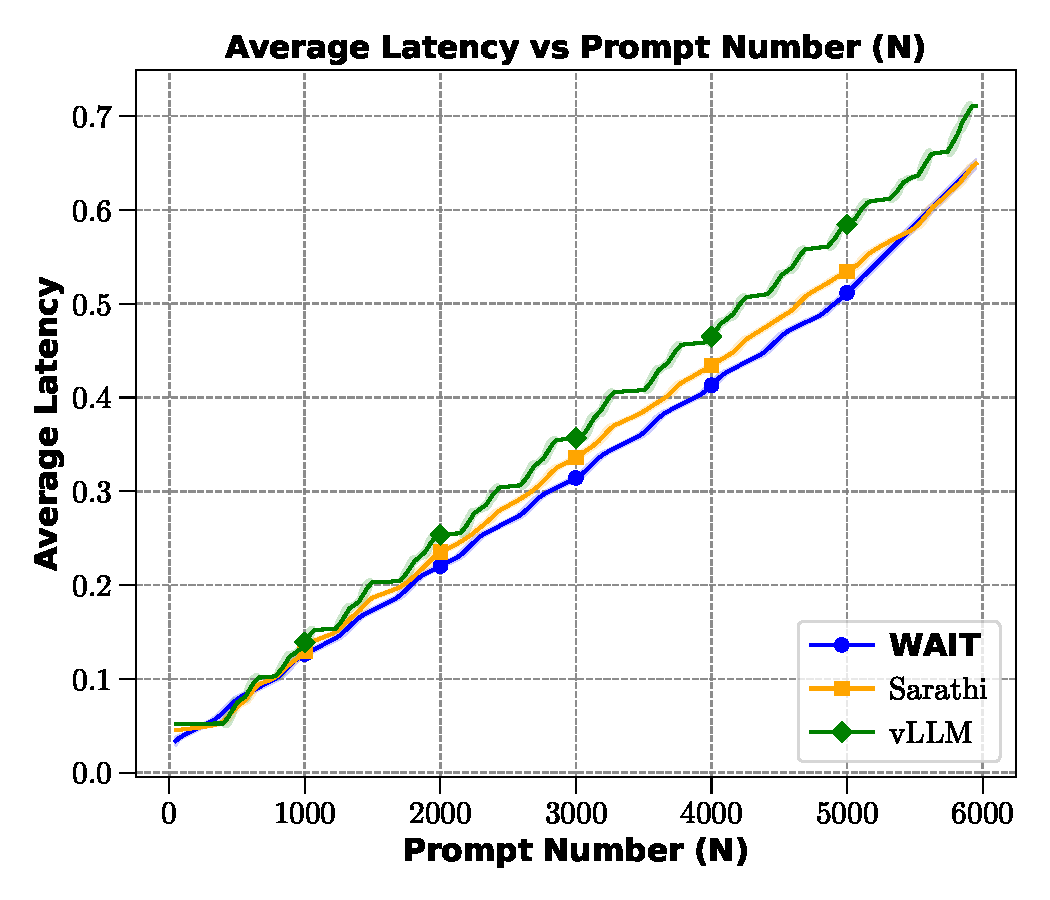
\includegraphics[width=\textwidth]{Experiments_pdf/test13_simulated_short_decode_bs=448_latency.pdf}
    \end{minipage}
    \caption{Average throughput and latency across algorithms on the synthetic dataset with high demand.}
    \label{fig:comparison WAIT long decode}
\end{figure}

\subsection{Experiment on Nested WAIT Algorithm}
Next, we evaluate the Nested WAIT algorithm, designed for scenarios where prompt output lengths are unknown. We test it on both synthetic and real-world datasets, using the same batch size limits across all algorithms and setting thresholds proportional to arrival rates in each segment for practical implementation.

We begin with a synthetic dataset where \( m=4 \), prefill lengths are fixed at 10 tokens, decode lengths are \( (20, 40, 80, 160) \), and arrival rates follow a \( 20:40:80:160 \) ratio. We set thresholds \( (n_1, n_2, n_3, n_4) \) with the ratio \( 15:14:12:8 \). Figure \ref{fig:comparison Nested WAIT, short prefill} shows improved throughput and latency over benchmarks.

For real-world testing, we use the dataset from \cite{zheng2023lmsys}, which contains over 210,000 prompts from Vicuna and Chatbot Arena. In this dataset, we use questions as prompts and answers as decoded tokens. Figure \ref{fig:distribution} shows the distribution of prefill and decode lengths. We randomly sample 50,000 prompts and simulate arrivals via a Poisson process.

To implement Nested WAIT, we group decode lengths (1 to 500 tokens) into 10 bins of 50 tokens each (e.g., [1-50], [51-100], etc). For each bin, we compute the mean prefill length (approximately 60 tokens, as shown in Figure \ref{fig:group}) and arrival rates proportional to \( 23:11:8:7:6:4:3:2:1:1 \). We set \( m=10 \) and thresholds \( (n_1, \dots, n_{10}) \) with the ratio \( 66:43:32:24:17:11:7:4:2:1 \), following \eqref{eq:nested_wait_thresholds}. Prompts in the \( k \)-th decode stage are assigned to segment \( \lceil k/50 \rceil \).
% More discussions on this segment design are left in Appendix \ref{sec:extension}.

We first test a synthetic workload with prefill fixed at 60 tokens and decode lengths clustered into 10 types (50, 100, ..., 500 tokens), with arrival rates matching the real dataset's proportions. We evaluate Nested WAIT with queries per second (QPS) of 55 and 550, shown in Figure \ref{fig:comparison_Nested_WAIT_real_world_low} and Figure \ref{fig:comparison Nested WAIT, real world, higher rate}, respectively. Nested WAIT outperforms benchmarks in both throughput and latency.

% \gan{Maybe, we can say that the Figure \ref{fig:comparison_Nested_WAIT_real_world_low} and Figure \ref{fig:comparison Nested WAIT, real world, higher rate} are on static arrival rate, and Figure \ref{fig:comparison Nested WAIT, real world} is on time-varying arrival rate bt with static threshold, which leads to a little latency overflow.}

Finally, we test the real dataset with original prefill and decode lengths, using the same thresholds. Figure \ref{fig:comparison Nested WAIT, real world} shows that Nested WAIT achieves higher throughput with a modest increase in latency (approximately 0.5 seconds per prompt), enhancing system efficiency while maintaining responsiveness. We applied the thresholds, originally designed for static arrival rates, to this time-varying scenario, which resulted in slightly higher latency.

\begin{figure}[ht]
    \centering
    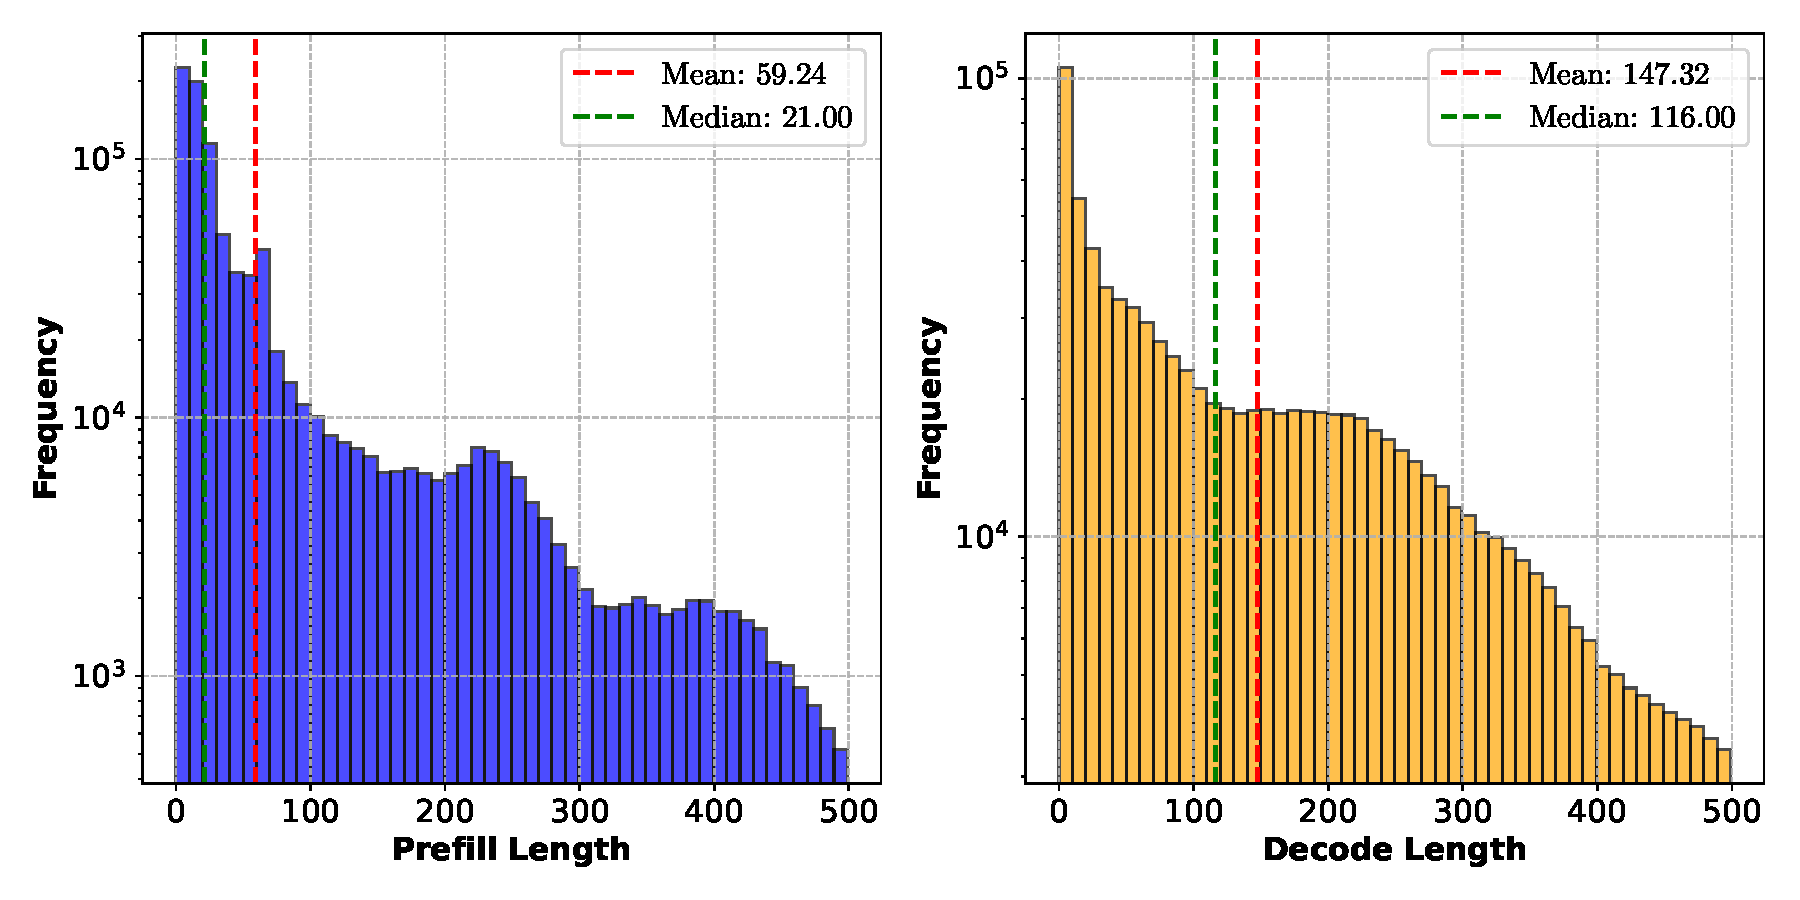
\includegraphics[width=0.6\textwidth]{Experiments_pdf/question_answer_lengths_distribution.pdf}
    \caption{Distribution of prefill and decode lengths in the real dataset.}
    \label{fig:distribution}
\end{figure}

\begin{figure}[ht]
    \centering
    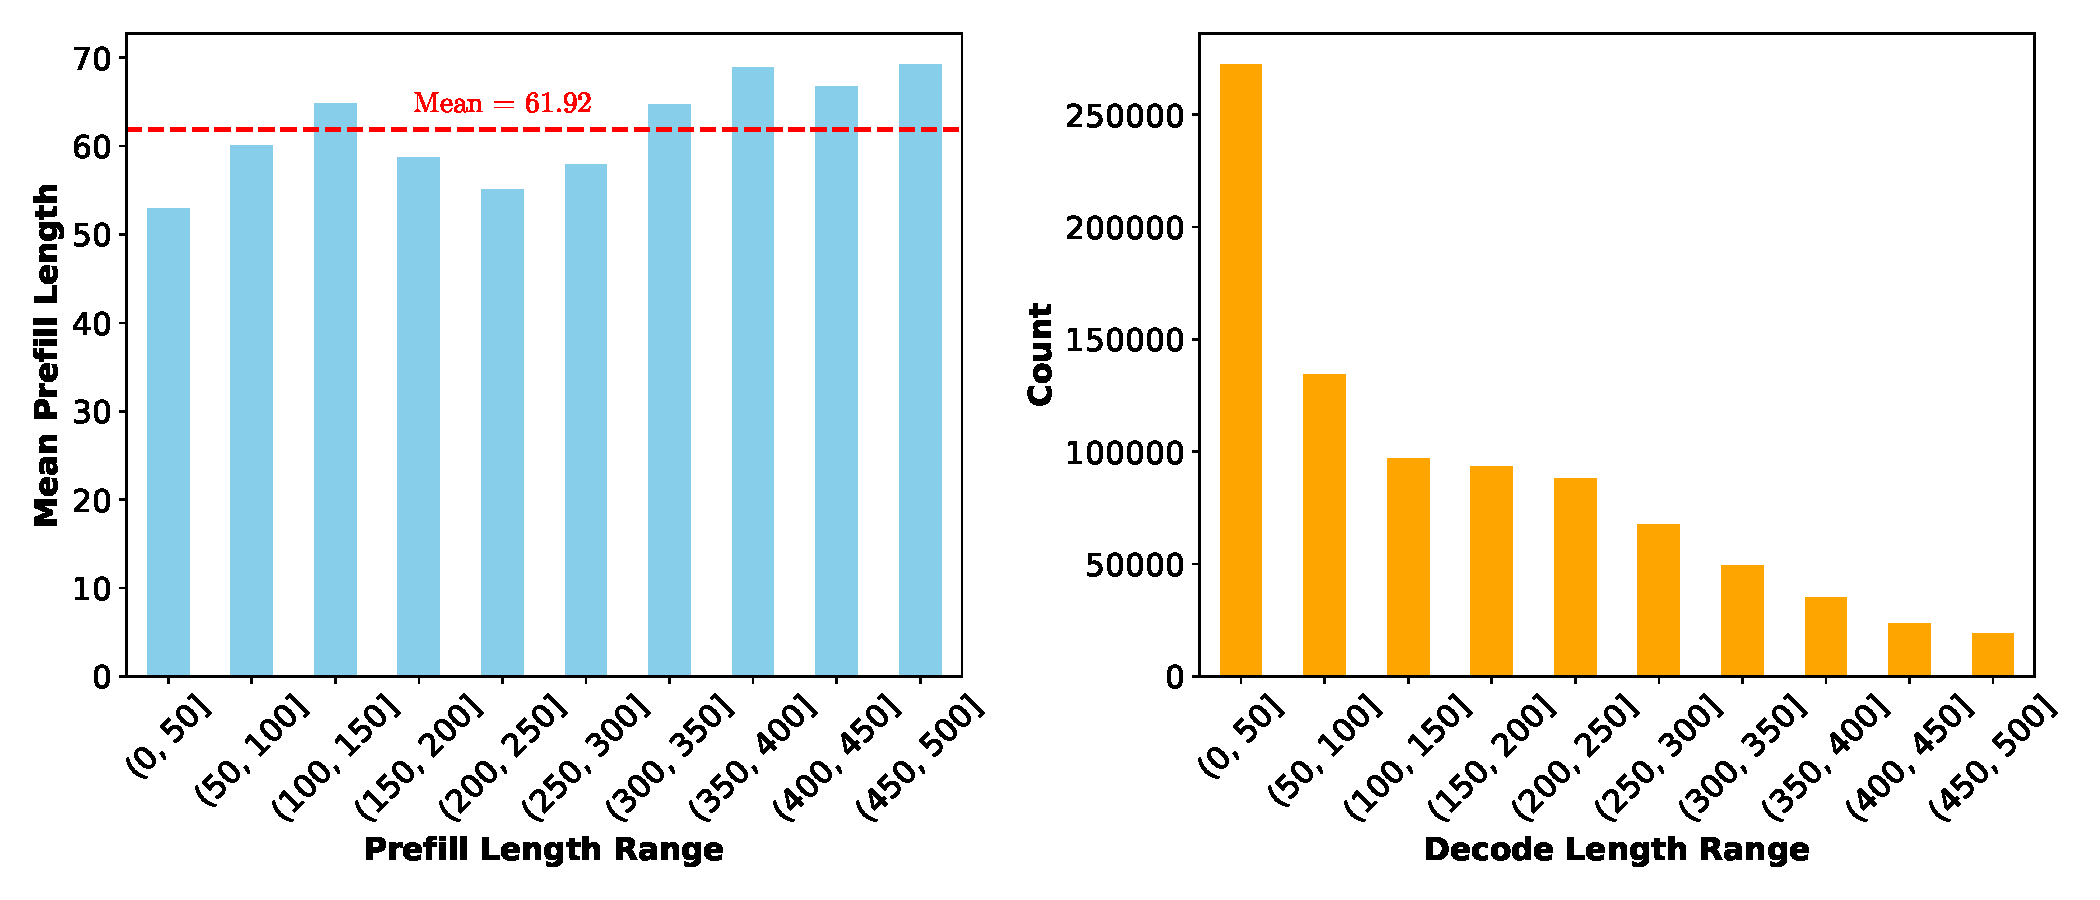
\includegraphics[width=0.6\textwidth]{Experiments_pdf/group.pdf}
    \caption{Mean prefill lengths and prompt counts per decode length bin in the real dataset.}
    \label{fig:group}
\end{figure}

\begin{figure}[htbp]
    \centering
    \begin{minipage}{0.4\textwidth}
        \centering
        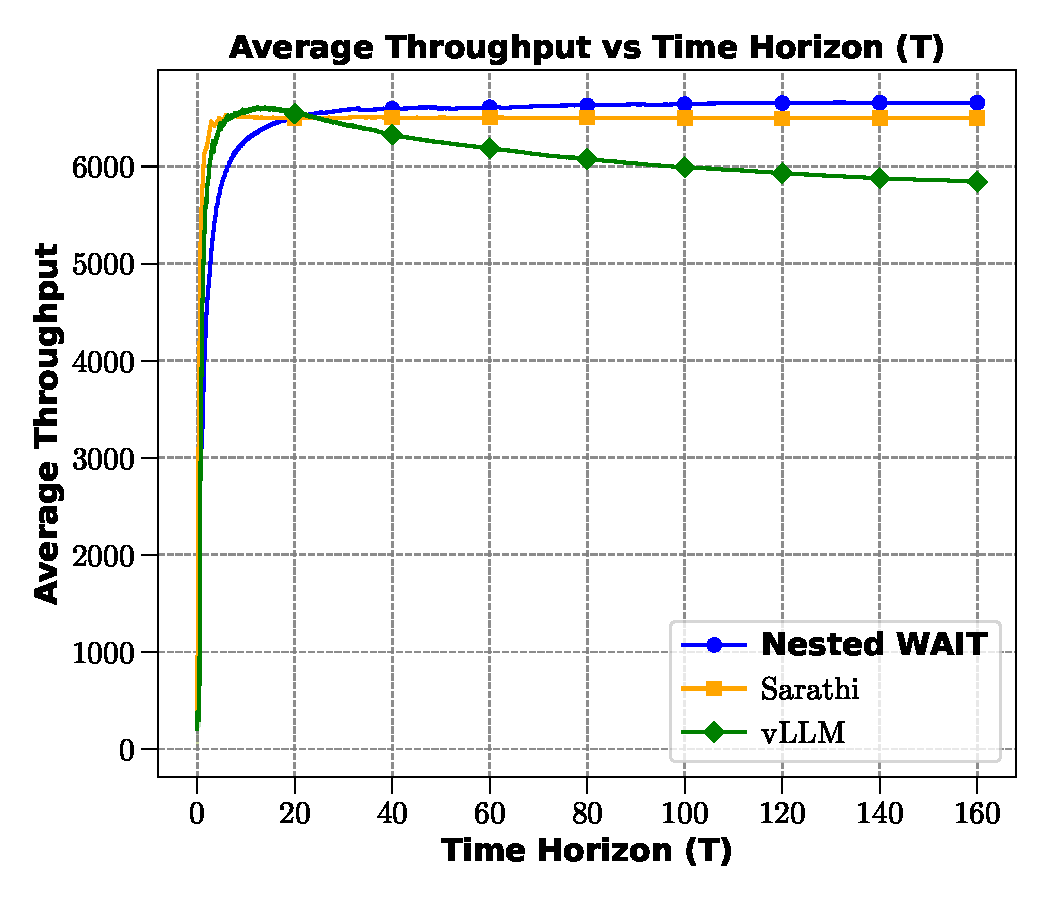
\includegraphics[width=\textwidth]{Experiments_pdf/test30_simulated_short_decode_bs=128_nested_real_not_trace_throughput.pdf}
    \end{minipage}
    \hfill
    \begin{minipage}{0.4\textwidth}
        \centering
        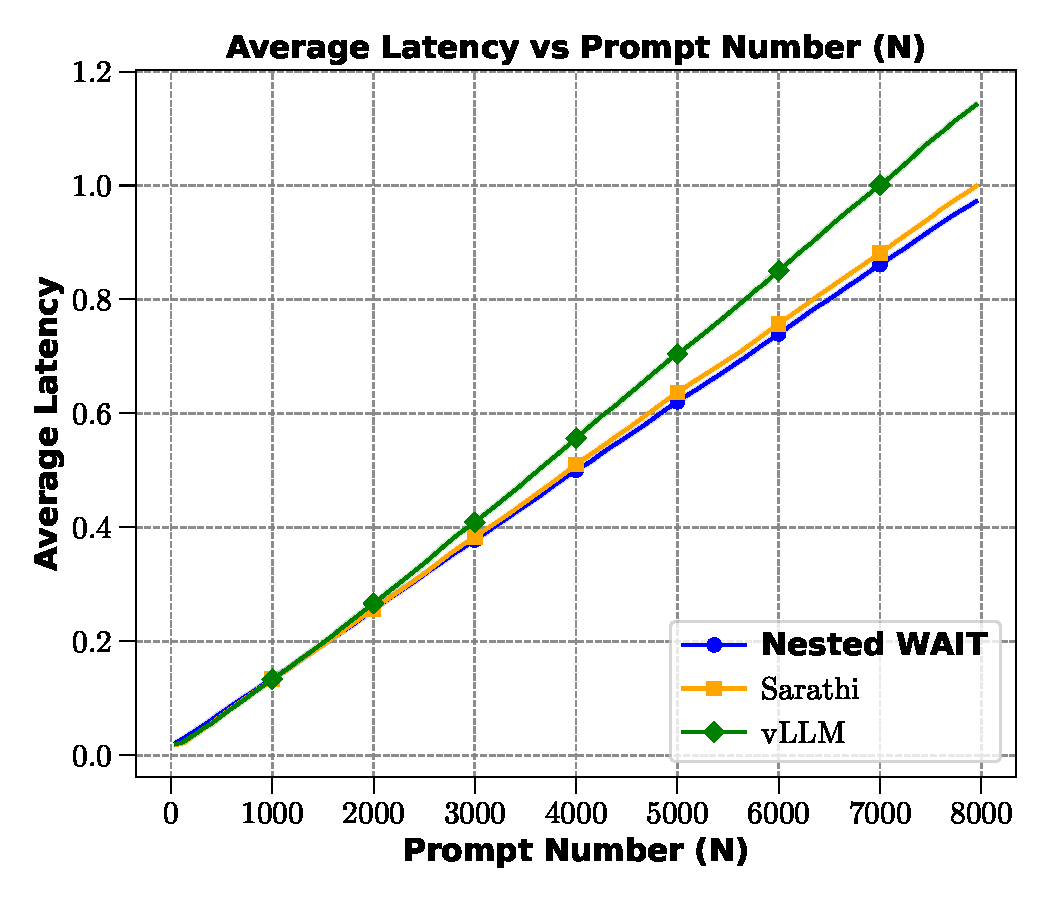
\includegraphics[width=\textwidth]{Experiments_pdf/test30_simulated_short_decode_bs=128_nested_real_not_trace_latency.pdf}
    \end{minipage}
    \caption{Average throughput and latency across algorithms on the synthetic dataset.}
    \label{fig:comparison Nested WAIT, short prefill}
\end{figure}

\begin{figure}[htbp]
    \centering
    \begin{minipage}{0.4\textwidth}
        \centering
        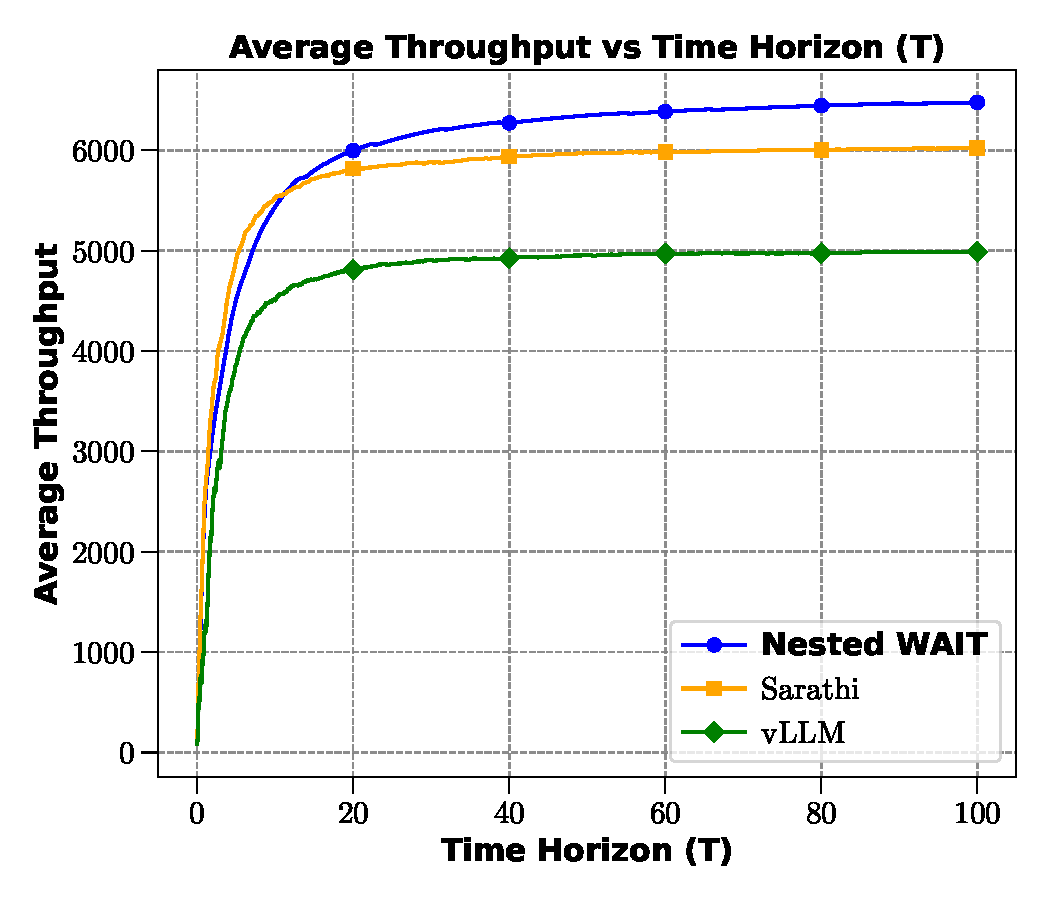
\includegraphics[width=\textwidth]{Experiments_pdf/test31_simulated_short_decode_bs=148_nested_real_not_trace_throughput.pdf}
    \end{minipage}
    \hfill
    \begin{minipage}{0.4\textwidth}
        \centering
        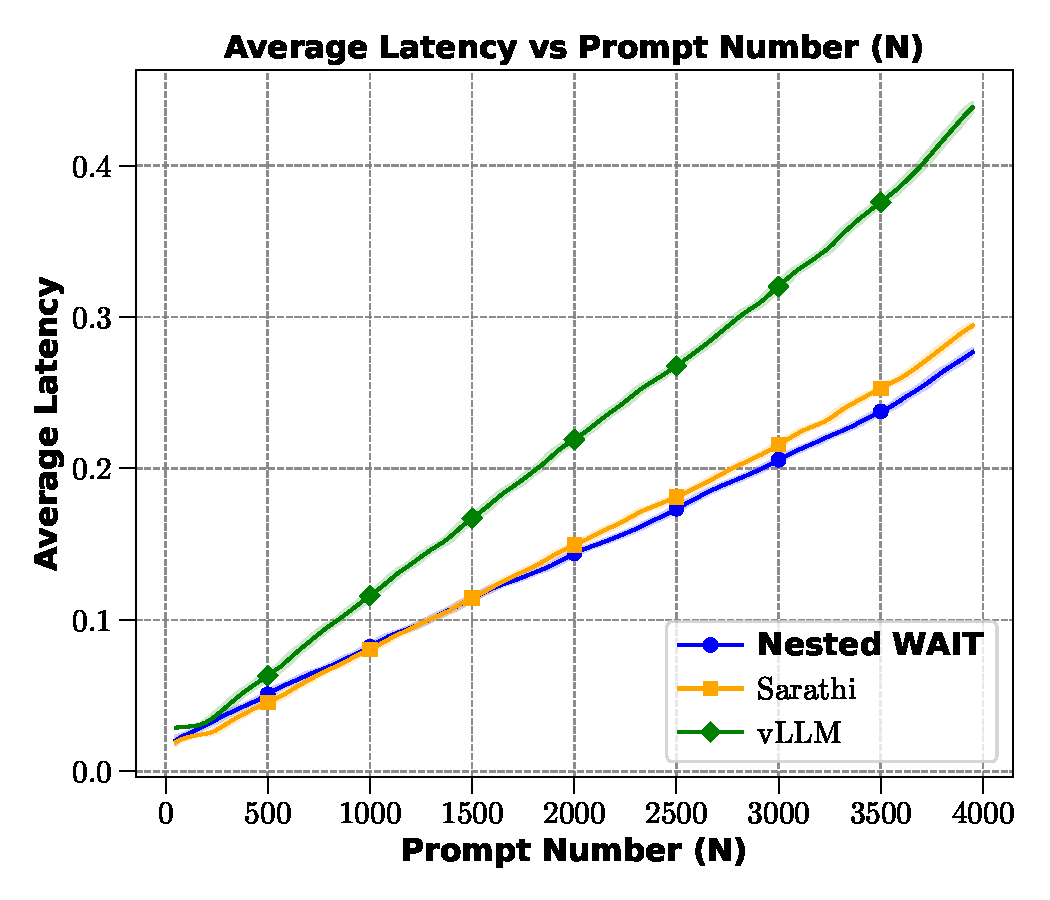
\includegraphics[width=\textwidth]{Experiments_pdf/test31_simulated_short_decode_bs=148_nested_real_not_trace_latency.pdf}
    \end{minipage}
    \caption{Average throughput and latency across algorithms on the real dataset with clustered output lengths (low arrival rates).}
    \label{fig:comparison_Nested_WAIT_real_world_low}
\end{figure}

\begin{figure}[htbp]
    \centering
    \begin{minipage}{0.4\textwidth}
        \centering
        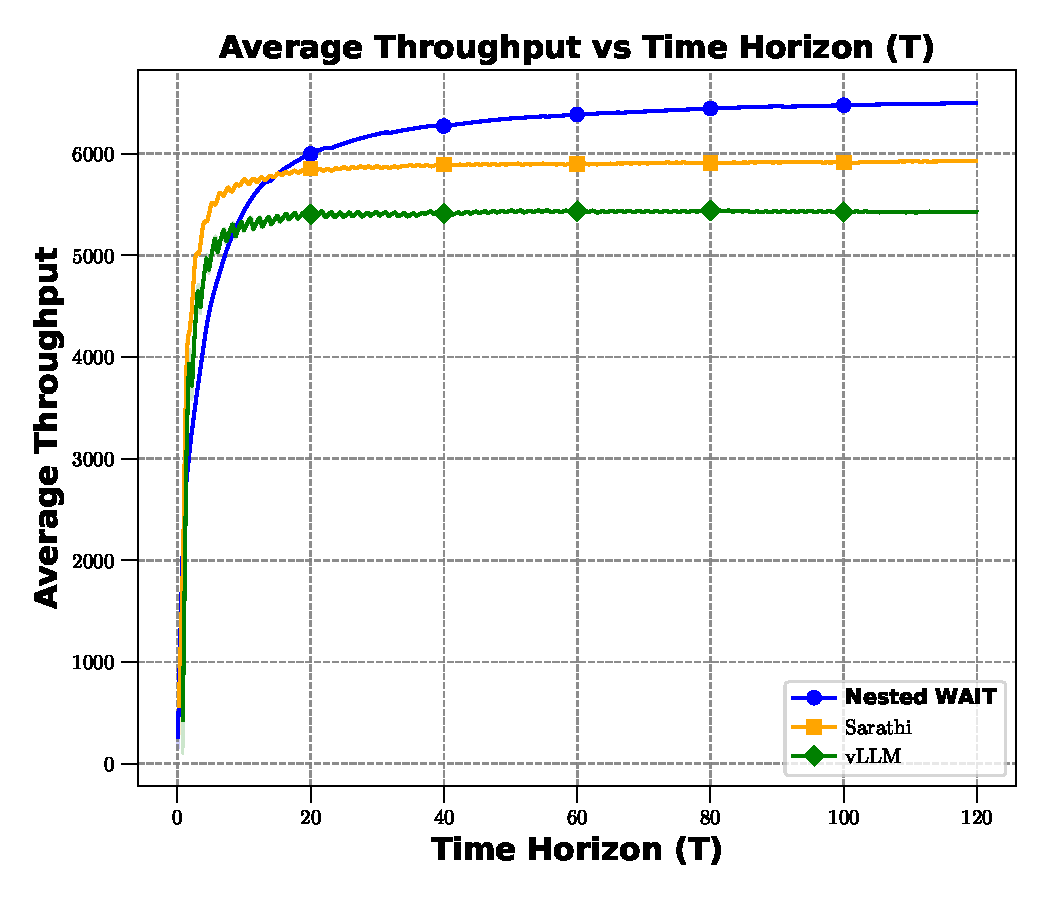
\includegraphics[width=\textwidth]{Experiments_pdf/test32_simulated_short_decode_bs=148_nested_real_not_trace_higher_rate_throughput.pdf}
    \end{minipage}
    \hfill
    \begin{minipage}{0.4\textwidth}
        \centering
        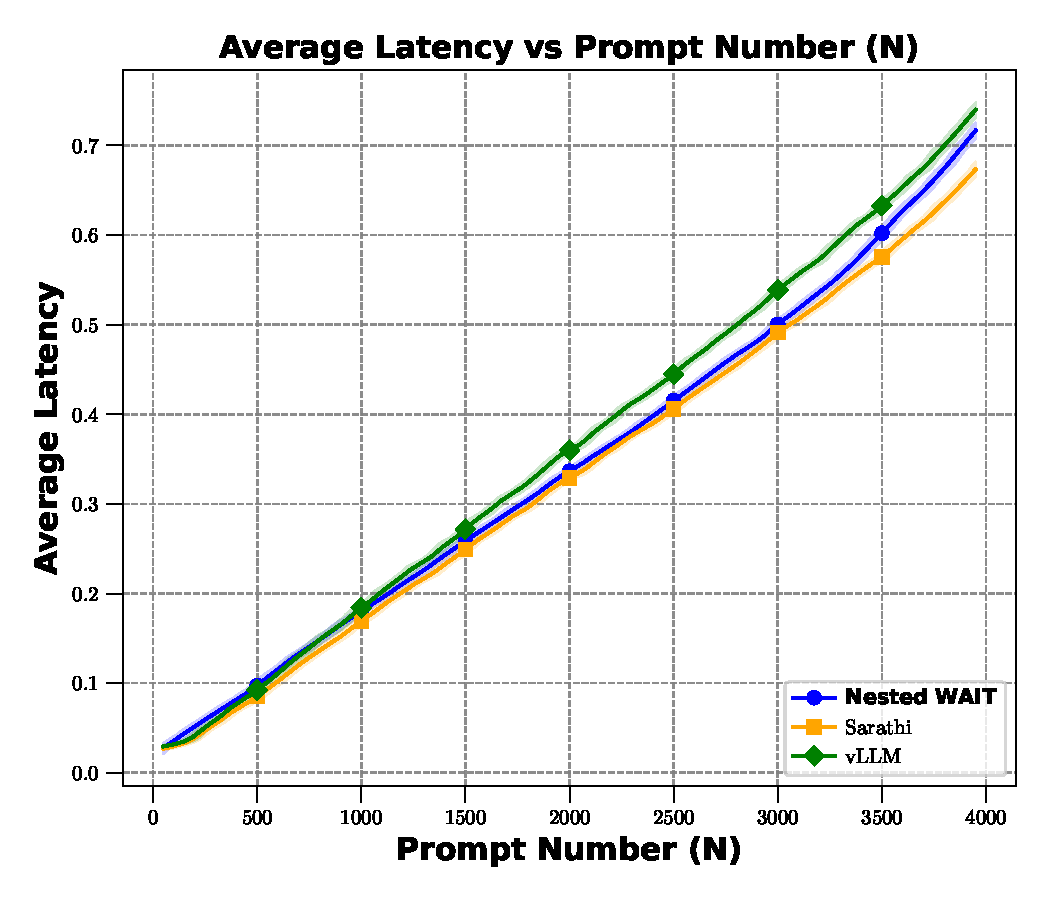
\includegraphics[width=\textwidth]{Experiments_pdf/test32_simulated_short_decode_bs=148_nested_real_not_trace_higher_rate_latency.pdf}
    \end{minipage}
    \caption{Average throughput and latency across algorithms on the real dataset with clustered output lengths (high arrival rates).}
    \label{fig:comparison Nested WAIT, real world, higher rate}
\end{figure}

\begin{figure}[htbp]
    \centering
    \begin{minipage}{0.4\textwidth}
        \centering
        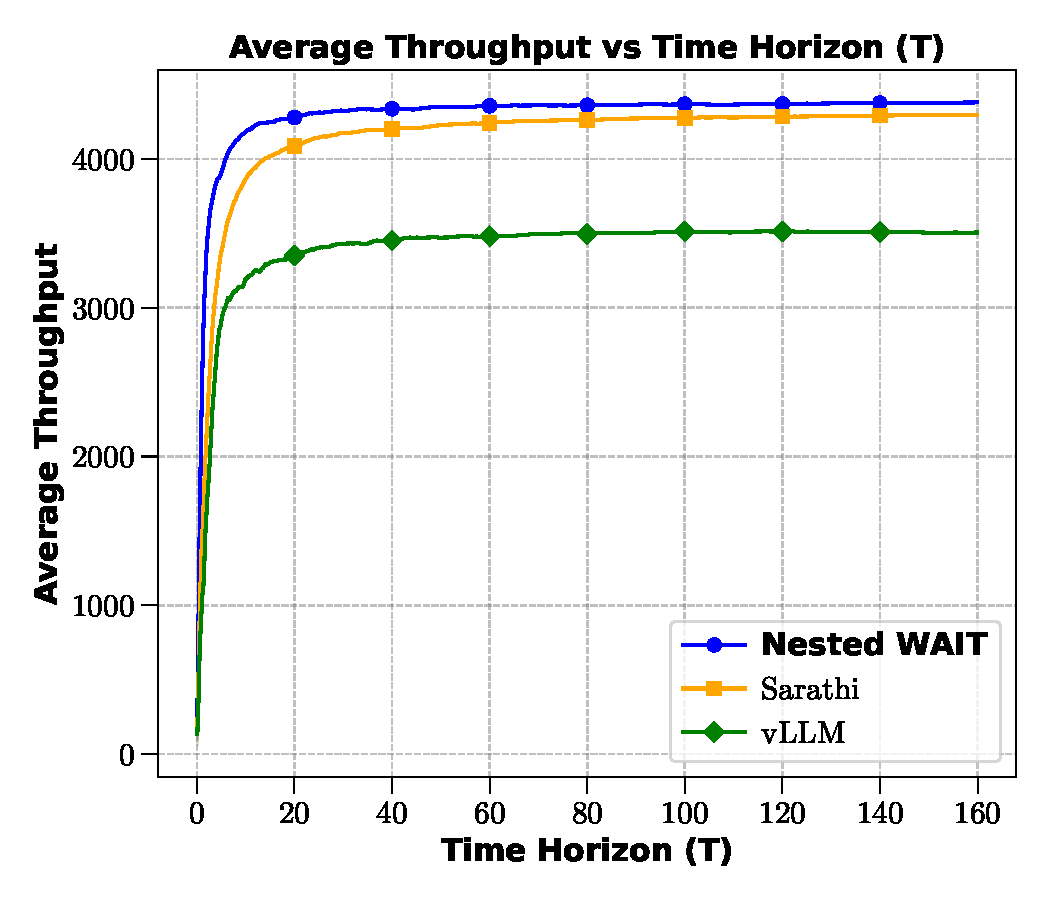
\includegraphics[width=\textwidth]{Experiments_pdf/test36_simulated_short_decode_bs=64_nested_real_TRACE_throughput.pdf}
    \end{minipage}
    \hfill
    \begin{minipage}{0.4\textwidth}
        \centering
        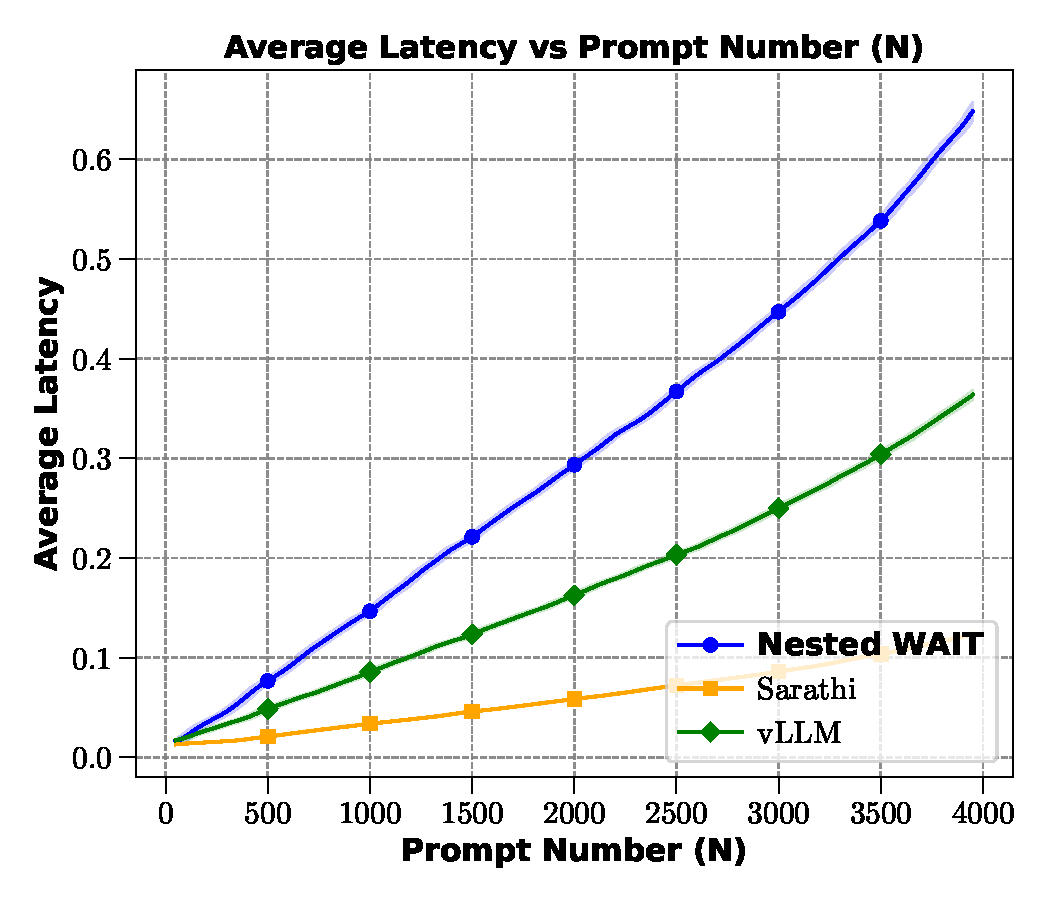
\includegraphics[width=\textwidth]{Experiments_pdf/test36_simulated_short_decode_bs=64_nested_real_TRACE_latency.pdf}
    \end{minipage}
    \caption{Average throughput and latency across algorithms on the real dataset with actual output lengths.}
    \label{fig:comparison Nested WAIT, real world}
\end{figure}